\section*{Vnímání}
\addcontentsline{toc}{section}{Vnímání}

Mezi podstatné funkce trezoru patří jeho vnímání veličin jako čas, jeho náklon nebo okolní tlak.
Deska proto obsahuje tři nebo čtyři, v závislosti na dostupnosti součástek, čipy které, které trezoru poskytují gyroskop, akcelerometr, magnetický kompas,
barometr a~RTC (Real Time Clock, hodiny reálného času). Díky těmto funkcím může trezor poskytnout možnost ovládání pomocí různých gest. Trezor třeba může 
sloužit, s~využitím magnetického kompasu a~lek kruhu, jako kompas, nebo se dá využít akcelerometr aby se dal trezor odemknout jen v konkrétním náklonu.
Všechny čipy zobrazené na obrázku [\ref{fig:E4-sch_vnimani}] komunikují s~ESP hlavně pomocí sběrnice I2C. Pro možnost zrychlení reakcí má však každý 
z~čipů také pin určení pro spuštění přerušení na procesoru. To je užitečné z~toho důvodu že komunikaci na I2C řídí ESP. Pokud se tedy ESP nerozhodne 
zeptat se jiného čipu na jím naměřené data, čip mu to nemá jak zdělit. Zároveň se však procesor nemůže bez ustání ptát na měření ostatních čipu 
protože by pak nestíhal dělat nic jiného. Proto jsou čipy vybaveny pinem který změní svou logickou hodnotu ve chvíli kdy naměřené hodnoty splní nějaké 
podmínky. 
Například muže být trezor naprogramován aby se otevřel v konkrétní čas, tento čas se potom dá nastavit v RTC jako hodnota které když RTC 
dosáhne přepne pin přerušení, a esp pak jen přečte logickou hodnotu pinu a nemusí komunikovat po I2C. % tuto větu by nebylo k zahození nakrouhat

\begin{figure}[htbp]
    \centering
    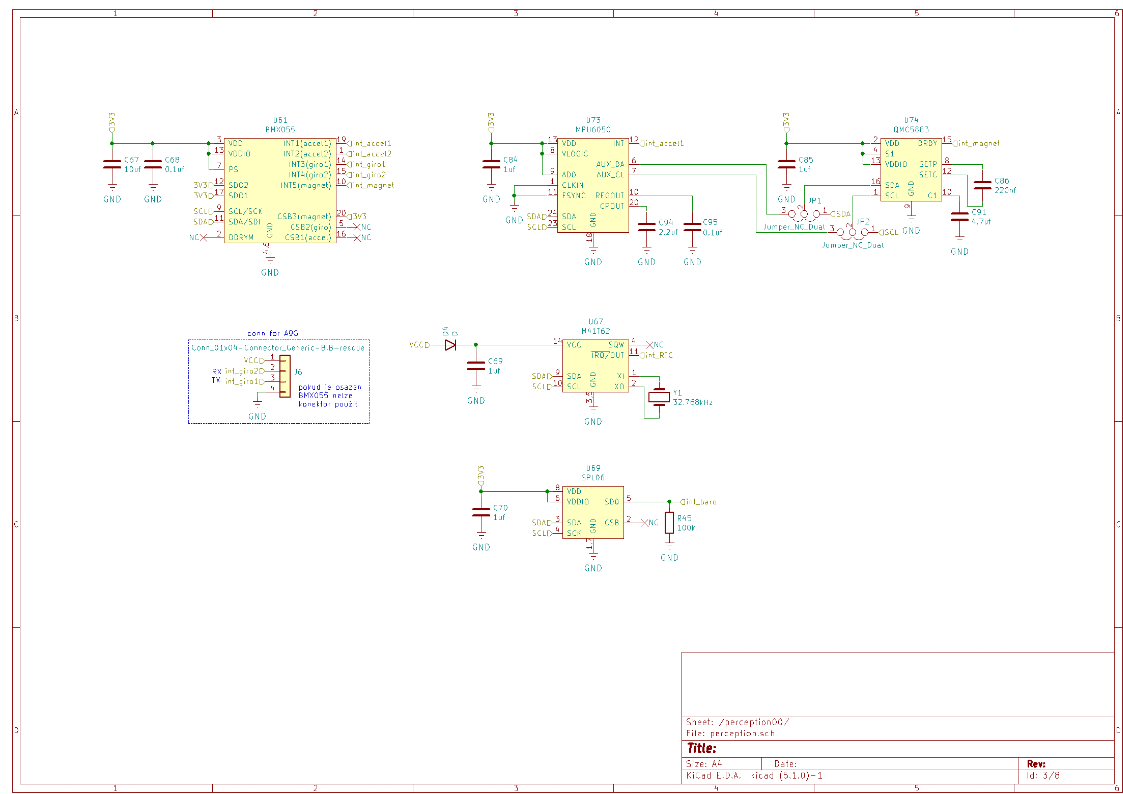
\includegraphics[width=\textwidth]{kapitoly/obrazky/E4/vnimani/sch.png}
    \caption{zapojení vnímacích čipu}
    \label{fig:E4-sch_vnimani}
\end{figure}

\paragraph*{Akcelerometr gyroskom a magnetický kompas}
\addcontentsline{toc}{paragraph}{Akcelerometr}
Na prvním prototypu verze E4 poskytoval akcelerometr, gyroskom i magnetický kompas čip \href{https://datasheet.lcsc.com/szlcsc/Bosch-Sensortec-BMX055_C94022.pdf}{BMX055}, protože však 
tento čip nebyl jednoduše dostupní přidal jsem na další verzi i čipi \href{https://datasheet.lcsc.com/szlcsc/TDK-InvenSense-MPU-6050_C24112.pdf}{MPU6050},
který obsahuje akcelerometr a gyroskop,
a \href{https://datasheet.lcsc.com/szlcsc/QST-QMC5883L-TR_C192585.pdf}{QMC5883} který akcelerometr poskytuje také. BMX055 neposkytuje jen tři osi 
akcelerometru ale obsahuje i tři osi gyroskopu a další tři magnetického kompasu. MPU6050 vedle toho poskytuje jen akcelerometr a gyroskop. 


\begin{figure}[htbp]
    \centering
    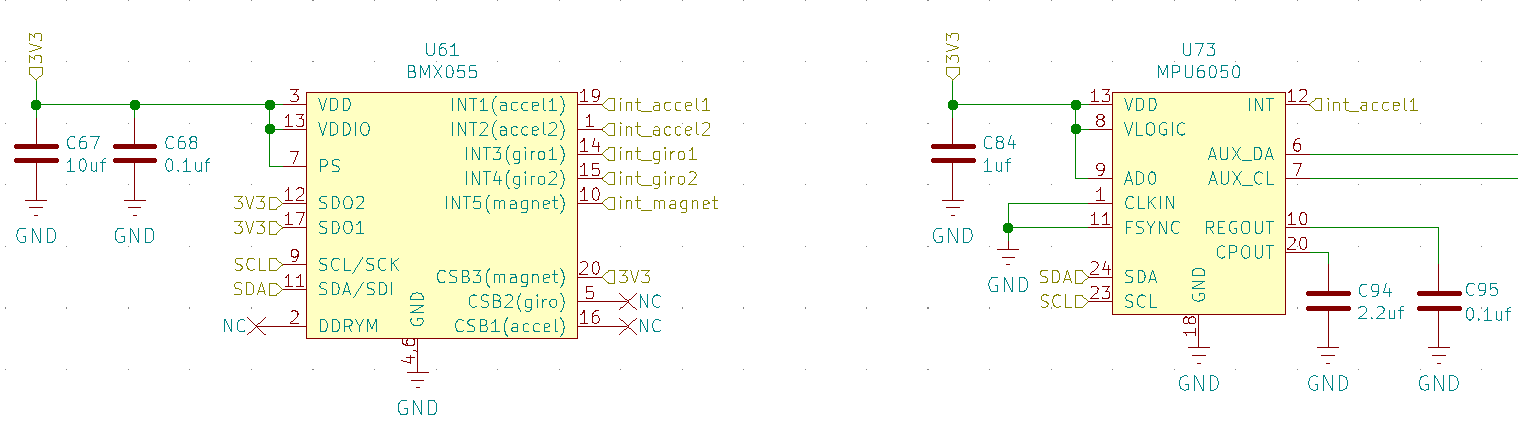
\includegraphics[width=\textwidth]{kapitoly/obrazky/E4/vnimani/BMX-MPU.png}
    \caption{zapojení čipů BMX055 a MPU6050}
    \label{fig:E4-step-up}
\end{figure}